% !TEX root = ./../main.tex
\chapter{Model of cell membrane and monolayer--protected NP}
\label{chap:tre}

\section{NanoParticle model}
Monolayer--protected metal \acp{NP} have the advantage of having a well defined molecular structure. That is, mono--dispersed solutions can be synthesized and structurally determined. In particular, \acp{NP} with a gold core can be stabilized by thiols\footnote{The thiol (R--SH) group is like the alcohol (R--OH) group but it is less polar respect to the second due the lower electronegativity of the sulfur respect to oxygen.}, which stably bind to the Au surface via Au-S bonds. 
%Thiolated \acp{AuNP} are air stable, electrochemically stable and thermally stable compounds [].
Several stable thiolated \acp{AuNP} are identified, differing in size of the gold core and number of ligands. In particular we consider a {Au$_{144}$(SR)$_{60}$} thiolated \ac{AuNP}, where R is the aliphatic chains of the thiol compounds. 

Changing the composition of the aliphatic chains bonded to the thiol group different properties of the thiolated \ac{AuNP} can be achieved, such as different net charge, different level of hydrophobicity, different size and so on. In particular, as we shall see, in the model we will use we consider only \ac{OT} and \ac{MUS} ligands that cover the \ac{AuNP} core with a monolayer in different composition and different surface arrangement. To overcome the computational cost of an atomistic model we use a \martini \ac{CG} model of the \ac{OT} and \ac{MUS} ligands. 

The model of the \ac{AuNP} and the \martini model of the \ac{OT} and \ac{MUS} ligands are developed by Federica Simonelli \etal\, in \cite{ourPaper}, and the reader is addressed to it for a more detail discussion about the model and the parameterization.

% gold core --> Thyiol passivated --> ligands
%Ligand Composition: Patched (1:1), Random (1:1) (1:2)
%Different level of hydrophobicity
%Different ligand charge: anionic/cationic NP

\subsection{Passivated gold core}
The gold core is composed of $144$ atoms which displays icosahedral symmetry and it is made of three bulk shell with $12$, $42$ and $60$ atoms, respectively. A surface shell of $30$ atoms completes the gold cluster structure. Then $60$ sulphur atoms, which blind the aliphatic chains (R) to the gold core, are bounded to the gold atoms on the surface through the typical bond structure RS--Au--SR. The shell construction is shown in figure~(\ref{fig:goldShell}).
\begin{figure}[!ht]
	\centering
	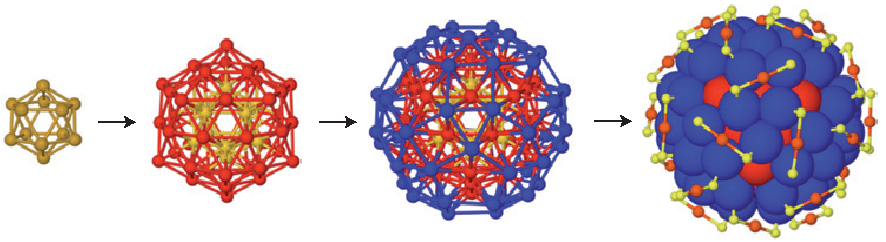
\includegraphics[width=0.8\textwidth]{./img/goldShell}
	\caption{First three frame: the concentric $12$--(yellow), $42$--(red) and $60$--(blue) atom gold internal shell, surrounded (last frame) by $30$ gold (red small) and $60$ sulphur (yellow small) surface atoms. The R chains is not shown. Taken from \cite{corePassivated}.}
	\label{fig:goldShell}
\end{figure}

The resulting diameter of the gold core is about $2$~nm. When passivated by thiols, its overall size depends on the length of the aliphatic chains bound to the sulphur atoms. The monolayer--protected \ac{AuNP} we will consider have a total diameter of about $4$~nm.

\paragraph{\textbf{gold elastic network}} Despite the computational cost associated to atomistically describe the gold cluster, all gold atoms are taken into account in order to allow us future studies on heating effect on lipid bilayer. Thus the bonds between gold atoms are allowed to vibrate. As we have seen in a previous section, a many--body potential should be used. Instead, as we are interested in the vibrational modes of the core atoms, 
%Federica Simonelli in her thesis work, found that
a more efficient way is to use an elastic network associate the potential energy
\begin{equation*}
	U = \frac{1}{2}\sum_i \sum_{j\ne i}k_{ij}(r_{ij} - r_{ij}^0)^2
\end{equation*}
where $r_{ij}$ is the distance and $k_{ij}$ is the bond constant for $i-j$ atom pair. 
%The bond constants is assigned so as to reproduce the vibrational spectrum of the gold core as provided by the many--body Gupta potential. 
The bond constant is assigned to $k = 32500$~kJ/(mol\,nm$^2$) for surface atoms and $k = 11000$ kJ/(mol\ nm$^2$) for bulk atoms. While the equilibrium distances are derived from []. A gold atom is considered as bulk atom if it has at least nine gold atom neighbors otherwise as a surface atom. A gold atom is considered neighbor to another if it lie within a shell of radius $0.35$~nm centered to the considered atom. In figure~(\ref{fig:goldNetwork}) the gold elastic network is shown.
\begin{SCfigure}[][hb]
	\centering
	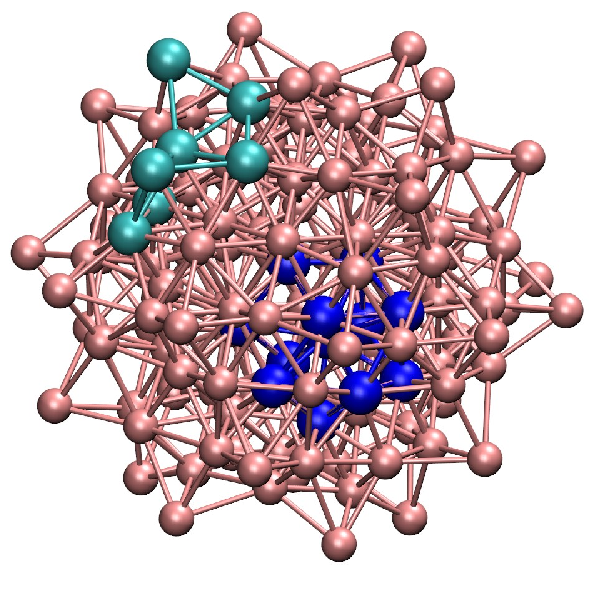
\includegraphics[width=0.35\textwidth]{./img/goldNetwork}
	\caption{Elastic network, represented by the stick bond, among gold atoms (pink). In cyan a surface atoms and its neighbors. In blue a group of bulk atoms and its neighbors. Taken from \cite{simonelliThesis}.}
	\label{fig:goldNetwork}
\end{SCfigure}

\paragraph{\textbf{sulfur elastic network}} An elastic network with bond constant of $1250$~kJ/(mol\,nm$^2$) is also used to model sulphur atoms on the surface of the \ac{NP} cluster with a cutoff distance of $0.55$~nm to select the sulphur neighbor atoms. The interaction between a sulphur atom and its nearest gold atoms is modeled through a harmonic potential with a bond constant of $32500$~kJ/(mol\,nm$^2$) and equilibrium distances given by []. In order to prevent the penetration of the sulphur atoms into gold core, a repulsive potential of the form $C/r^{-12}$ where $C = 0.92953\cdot 10^{-6}$~(kJ\,nm$^{12}$)/mol models the non--bonded interaction between gold and sulphur atoms which are not involved in any of the previous bonds. In figure~(\ref{fig:NPCluster}) sulphur passivated \ac{AuNP} cluster with the complete elastic network is shown. 
%For a more comprehensive discussion about the parameterization and the model of the \ac{AuNP} core the reader is addressed to thesis work of Federica Simonelli \cite{ourPaper}.
\begin{SCfigure}[][h]
	\centering
	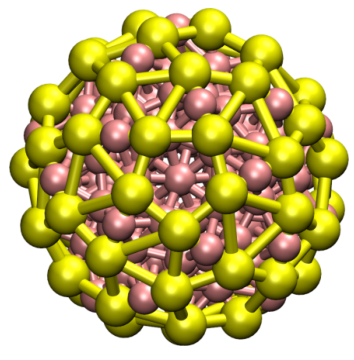
\includegraphics[width=0.35\textwidth]{./img/NPCluster}
	\caption{The \acs{AuNP} cluster. Gold atoms are in pink and sulfur atoms in yellow. The elastic network for both gold and sulfur atoms are represented by sticks. Taken from \cite{ourPaper}.}
	\label{fig:NPCluster}
\end{SCfigure}

% some information about gold core: dimensions, number of atoms, model used, elastic network, shel construction

\subsection{Functionalizing ligands}
Our \ac{AuNP} core is functionalized with \ac{MUS} and \ac{OT} ligands. The former is a charged compounds made of eleven \ac{CH2} groups and a charged terminal \ac{SO4-} group. The charged terminal group make it partially hydrophilic. The latter, instead, is completely hydrophobic and it is made by seven \ac{CH2} groups and one \ac{CH3} terminal group. Using both hydrophilic and hydrophobic groups guarantees that such \acp{NP} are stable, that is, does not aggregate, in both aqueous and non--aqueous environments.

%\subsection{OT ligands}
\paragraph{\textbf{OT Model}} Two \martini beds of type C$_1$ model the eight carbon atoms of the \ac{OT} backbone and their hydrogen atoms. The chemical structure and the resulting \ac{CG} \martini model is shown in figure~(\ref{fig:ot}). The first bead of each \ac{OT} ligands is bound to a sulphur atom via a harmonic potential with a bond constant of $1250$~kJ/(mol\,nm$^2$) and equilibrium length of $0.47$~nm. The second bead is connected to the first by same bond potential. An angle potential as in equation~\eqref{eq:martiniAngle} is used among the three particles. Parameters are fixed in accordance with the standard \martini ones (see section~\ref{sec:martiniPotential}). Moreover a purely repulsion potential, as described in the previous section, is used between C$_1$ beads and gold and sulfur atoms to prevent the co--penetration.
\begin{figure}[!ht]
	\centering
	\subfloat[\acs{OT} ligand]{%
		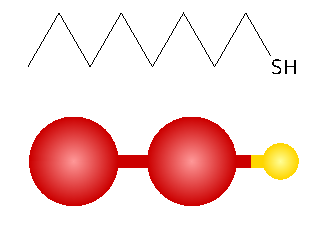
\includegraphics[width=0.3\textwidth]{./img/OT/OT}%
		\label{fig:ot}%
	}%
	\qquad\qquad%
	\subfloat[\acs{MUS} ligand]{%
		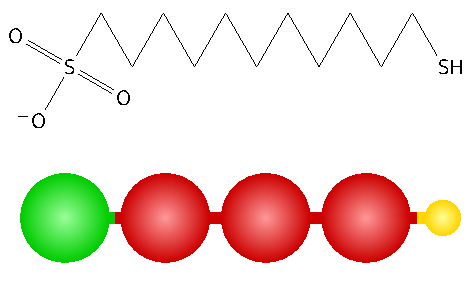
\includegraphics[width=0.35\textwidth]{./img/MUS/MUS}%
		\label{fig:mus}%
	}%
	\caption{Top: chemical structure. Bottom: \acs{CG} \martini model (red: C$_1$ bead, green: Q$_\text{da}$ negatively charged bead and yellow: sulfur atom).}
\end{figure}

%\subsubsection{MUS ligands} %Anionic an the cationic???
\paragraph{\textbf{MUS Model}} Three \martini beads of type C$_1$ model the hydrophobic chain even if one of them groups three carbon atoms instead of four. The charged group is modeled as a Q$_\text{da}$ beads with a charge of $-\mathsf{e}$. The chemical structure and the resulting \ac{CG} \martini model is shown in figure~(\ref{fig:mus}). Even in this case the first bead of a \ac{MUS} ligand is bounded to the sulphur atom through a harmonic potential with the same parameter: bond constant of $1250$~kJ/(mol\,nm$^2$) and equilibrium length of $0.47$~nm. The same potential is used to bind all other beads to the previous one. An angle potential as in equation~\eqref{eq:martiniAngle} is used among the sulfur atom, the first C$_1$ and second C$_1$, among the first, the second and the third C$_1$ beads and so on for all four beads. Parameters are fixed in accordance with the standard \martini ones (see section~\ref{sec:martiniPotential}). As in the \ac{OT} ligand model, a purely repulsion potential, as described in the previously, is used between C$_1$ beads and gold and sulfur atoms to prevent the co--penetration. The same applies between Q$_\text{da}$ bead and gold and sulfur atoms.

\paragraph{\textbf{level of hydrophobicity}} The \ac{AuNP} core can be functionalized with both ligands in different composition. In particular varying the ratio between the \ac{OT} and \ac{MUS} ligands different levels of hydrophobicity can be reached: it decrease augmenting the number of charged ligands. Two surface composition is considered: (\ac{MUS}:\ac{OT} $1$:$1$) and (2:1), but the former is the main used in this thesis work.

\paragraph{\textbf{surface arrangements}} The arrangements of the ligands on the \ac{AuNP} surface can be made in two possible way: randomly or with a predetermined scheme. In particular for the second possibility we use a striped scheme: the \ac{NP} surface is divided in three strip, the external two stripes are cover with \ac{MUS} ligands while the central with \ac{OT} ligands. For this thesis work we consider three type of \ac{NP}: striped (\ac{MUS}:\ac{OT} $1$:$1$), random (\ac{MUS}:\ac{OT} $1$:$1$) and random (\ac{MUS}:\ac{OT} $2$:$1$). In figure~(\ref{fig:coating}) the different coatings for the \ac{NP} core is shown.

\begin{figure}[!ht]
	\centering
	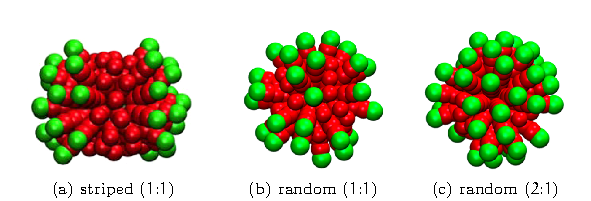
\includegraphics[width=0.9\textwidth]{./img/coatings/coat}
	\caption{Au\acs{NP} with different ligands surface arrangements and composition. From left to right: striped (\ac{MUS}:\ac{OT} $1$:$1$), random (\ac{MUS}:\ac{OT} $1$:$1$) and random (\ac{MUS}:\ac{OT} $2$:$1$). Hydrophobic beads are shown in red while the negatively charged beads are green.}
	\label{fig:coating}
\end{figure}

%\section{Model biological membrane}

\section{Real cell membranes}
The cel membrane or cytoplasmic membrane is a biological membrane that separate the interior and the external environments of a living cells. The basic function is to protect cells from its surroundings but it also takes the function of a ``customs'' in order to allow the cells to exchange chemical compounds from and to the external environments. To fulfill at this role the cell membrane is a crowded environments consisting of phospholipids, glycolipids, carbohydrates proteins and so on as we can see from figure~(\ref{fig:cellMembrane}).
\begin{figure}[!ht]
	\centering
	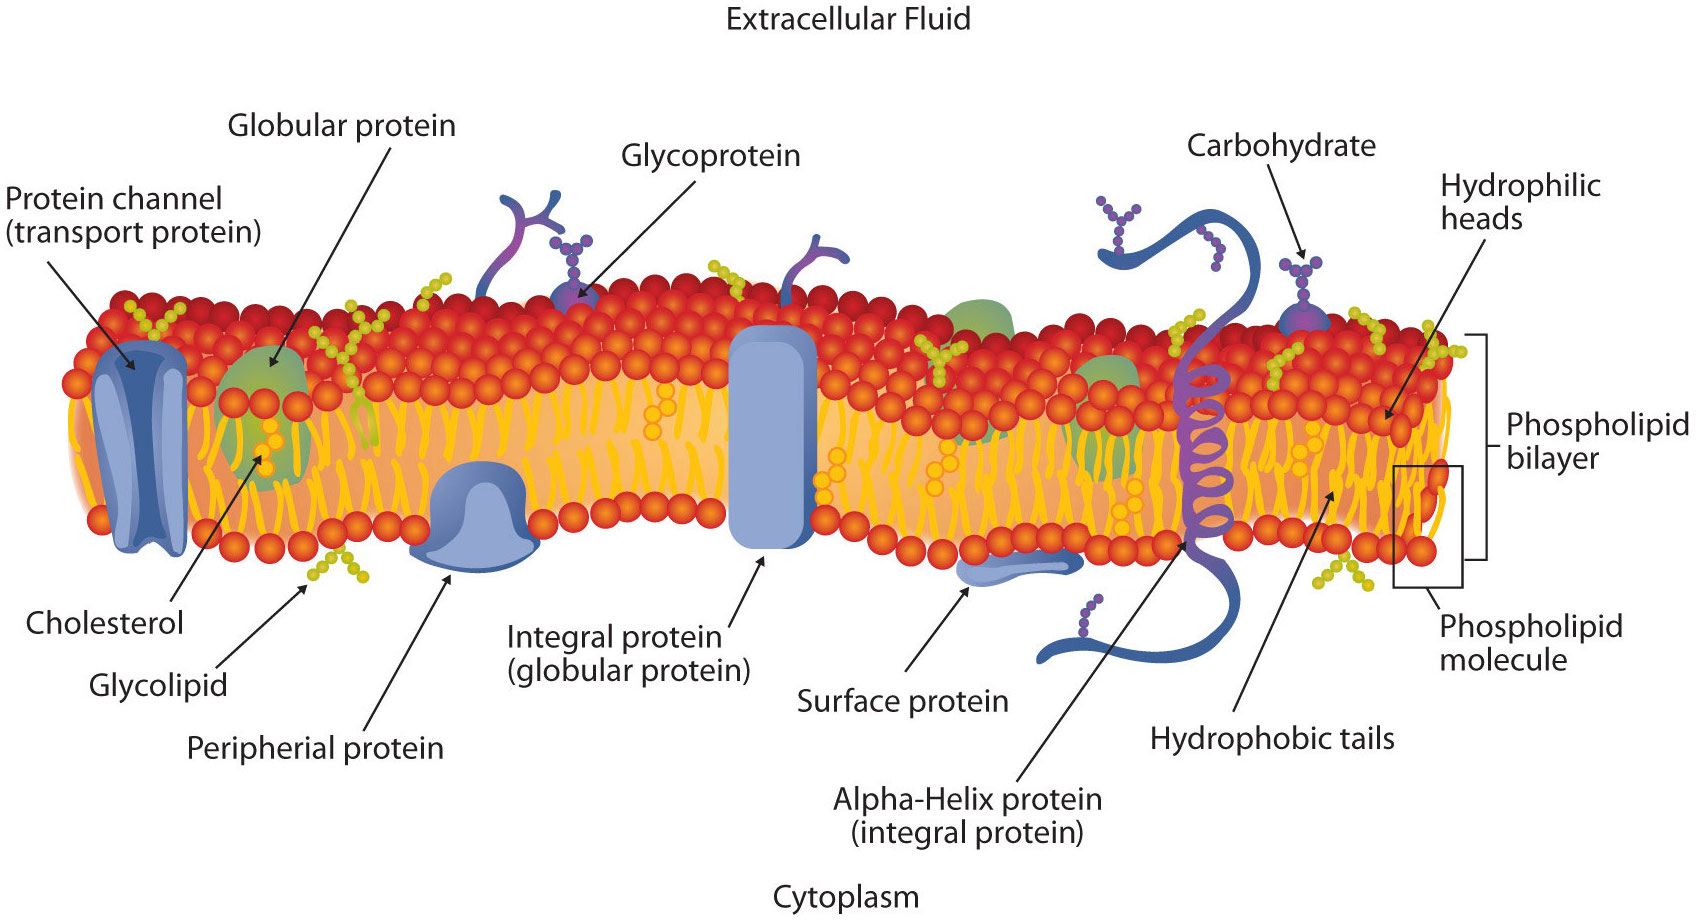
\includegraphics[width=0.9\textwidth]{./img/cellMembrane}
	\caption{Schematic representation of a biological cell membrane.}
	\label{fig:cellMembrane}
\end{figure}

The skeleton of a cell membrane is a bilayer sheet made of \textit{phospholipids}. They are a kind of lipids made of a polar or charged head, which is hydrophilic and one or two fatty acid hydrocarbon chains, often called lipid tails, which are instead hydrophobic; phospholipids are then amphiphilic molecules. This amphiphilic nature play a key role in the bilayer formation. In fact the formation of a bilayer in water is a self--assembly process driven by the hydrophobic effect which acts so as to minimize the number of hydrophobic contact between water and lipids tails. Moreover the bilayer sheet is not the only possible structure, based on the concentration of the phospholipids in water and on the temperature the self--assembly process can lead to three main different structures: bilayer sheet, liposome and micelle. In figure~(\ref{fig:lipidsStructures}) a schematic representation of this three different structures is shown.
\begin{SCfigure}
	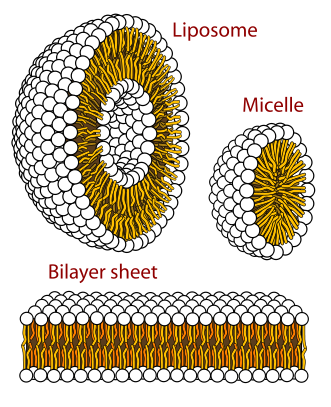
\includegraphics[width=0.3\textwidth]{./img/lipidsStructures}
	\caption{Cross--section view of the structures that can be formed by a self--assembly process of phospholipids in aqueous solution.}
	\label{fig:lipidsStructures}
\end{SCfigure}

A real lipid bilayer often contains hundred of different lipid species. They differ in the length of the hydrocarbon chains, in the degree of unsaturation, i.e. in the number of double bond in the hydrocarbon chains, and in different composition of the head that can be polar or non--polar. There two main classes of phospholipids that make a cell membrane of animals: glycerophospholipid (phosphatidyl--choline, phophatidyl--ethanolamine, phophatidyl--serine, phosphatidyl--serine ) and phosphosphingolipids (sphingomyelin). In the former group the lipid tails are bound to a glycerol group while the latter do not have glycerol and the lipid tails have a backbone of sphingoid bases, absent in the former. This five types take into account for more then half of the lipid in most membranes.

The cell membrane has a quasi--liquid properties at physiological temperature. This is in part due to some disorder in the alignment of the lipid tails produced by the presence of unsaturated chains. Another contribution arise from the area occupied by the lipid heads which determines the distance between the hydrocarbon chains. This fluid character make the lipid bilayer like a solvent in which the other molecules dissolved (lipids and protein) are free to diffuse. Moreover the lipids itself can move in different ways. The main movement and the associated time scale are summarized as follow
\begin{itemize}
	\item lipids conformational change (few nanoseconds);
	\item lipids protrusions out--of--plane (tens of picoseconds);
	\item diffuse within a leaflet (order of tens of nanoseconds);
	\item bilayer undulation and thickness involve collective motion of many lipids.
\end{itemize}
There are also many rare events that take place on the order of hours or even days, such like lipid flip--flop, in which a lipid go to the opposite leaflet; ions translocation; \textit{electroporation} by water, for example due to a cross membrane ions imbalance, in which water penetrate inside the bilayer and destroys a small portion in order to come to the other leaflet; water--helped ions permeation, called \textit{water--finger} and more general water defects inside the membrane.

For what concern the length scale, the bilayer thickness is determined by the length of the lipid tails and their degree of unsaturation. Typically the hydrophobic region is $\sim 3$~nm thick while each hydrophilic regions is $\sim 1$~nm thick. Hence the typical bilayer thickness is around $\sim 4\div 5$~nm.

\section{Model cell membranes}
As we have seen above, the cell membrane is an extremely complex environment due to the large number of different species and lipids which composes and resides in the bilayer sheet. The most common simplification in order to develop a model to use in a \ac{MD} simulations at atomistic or \ac{CG} level, consist to considers only one specie of phospholipid and no other compounds. In the bilayer model we will use in this thesis work, we consider model biological membrane consisting of \ac{POPC}. It is a zwitterionic glycerophospholipid of type phosphatidyl--choline whose head is made of a phosphate (PO$_4^-$) and a choline (C$_5$H$_{14}$NO$^+$) groups. It has two hydrocarbon chains: one is a saturated chain (palmitoyl) and the other is an unsaturated chain (oleoyl). The head groups and tails are both bounded to the glycerol group (C$_3$H$_8$O$_3$). In the top of figure~(\ref{fig:popc}) the chemical structure of the \ac{POPC} lipid is shown.

It is clear that the number of lipids that constitute a real cell membrane is enormous and it is extremely hard to take into account an entire cell membrane in a \ac{MD} simulation. A first approximation is to consider only a small area of the model bilayer. Given the medium area per lipid of about $0.65$~nm$^2$ and a portion of bilayer of $\sim 160$~nm$^2$, which corresponds to about $250$ lipids per leaflets, the total number of particles to be included in a atomistic simulations (excluding hydrogen atoms) are about $26000$ plus the water molecules. This has a very expensive computational cost and the range of phenomena which can be studied on these time and length scales is very limited, calling for the adoption of a \ac{CG} approach.

\begin{figure}[!ht]
	\centering
	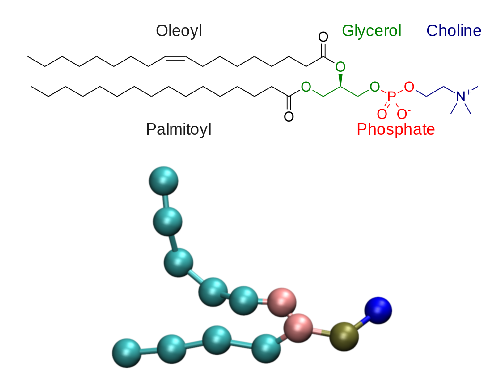
\includegraphics[width=0.7\textwidth]{./img/POPC/popc}
	\caption{Top: chemical structure of a \acs{POPC} lipid. Bottom: \martini \acs{CG} model. The tan bead is the phosphate group, choline is in blue, the two pink beads represents the glycerol group and the hydrophobic chains in cyan.}
	\label{fig:popc}
\end{figure}

\paragraph{\textbf{martini model}} As described in section \ref{sec:martini}, in this thesis work we use the \martini \ac{FF} for \ac{CG} lipids \cite{Martini}. The authors have developed a well suitable and comprehensive model about \ac{POPC} and a large variety of lipids. We consider a lipid bilayer made of $512$ \ac{POPC} lipids which extends on a surface of about $160$~nm$^2$ and whose thickness is about $4$~nm. The \martini model for the \ac{POPC} lipid maps the choline and the phosphate groups into two beads of type Q$_0$ and Q$_\text{a}$ negatively and positively charged, respectively. The saturated tail is modeled with four beads of type C$_1$ while the unsaturated tail is built up of four C$_1$ beads and one C$_3$ bead which corresponds to the unsaturated group of atoms. The glycerol group is modeled with two beads of type N$_\text{a}$. A comparison between the chemical structure and \ac{CG} model is shown in figure~(\ref{fig:popc}).

\paragraph{\textbf{model comparison}} The standard \martini \ac{FF} is able to capture the main aspects of the physical properties of a lipid bilayer with less computational effort respect to an atomistic simulation. These properties are the area per lipid, the lipid diffusion constant, the distribution of groups across the membrane, the bending and the area compression moduli, the stress profile across the membrane and many other as described in the original work by Marrink \etal\, \cite{Martini}. Nevertheless many other properties, prevalently mediated by the electrostatic interaction, are not well described. As we have seen in the previous Chapter this is because the \martini model does not take into account the long range treatment of the electrostatic interaction and because the standard \martini water is prevalently insensible to the electrostatic interaction\footnote{Moreover we can not forget that the \martini water bead takes into account four real water molecules. And hence the probability for a \martini water bead to permeate the hydrophobic region of the membrane is much less then for a water molecule in an atomistic \ac{FF}.}. To overcome to this problem the use of the \ac{PW} model and the \ac{PME} method, as outlined in \cite{MartiniReview} and \cite{PW}, are crucial to better describe the aforementioned process that involve lipid bilayer, water and charged ions. These are ions translocation; electroporation of the lipid membrane by water, due to a cross membrane ions imbalance; water--helped ions permeation and many other water defects inside the membrane as better described in the works of Marrink and Yesylevskyy.

\paragraph{\textbf{ions translocation}} An important phenomena mediated by the electrostatic interactions that is crucial for this thesis work is the lipid membrane ions translocation. In \cite{PW} the authors have computed the \ac{FES} of the translocation of Na$^+$ and Cl$^-$ ions\footnote{The \martini model for Na$^+$ and Cl$^-$ associates the ion plus the hydration shell to a bead of type Qd positively charged and Qa negatively charged, respectively.} across a \acs{DPPC} membrane using umbrella sampling and the \ac{WHAM} for the standard \martini model, with the use of the \ac{PW} and with \ac{PW} and \ac{PME} method. The height of the barriers are summarized in table~(\ref{tab:ionTranslocation}). The same \ac{FES} for a \acs{DMPC} membrane was calculated by Khavrutskii \etal\, \cite{atomisticTranslocation} with an atomistic \ac{FF}. Since the \martini model for the \acs{DPPC} lipid also model the \acs{DMPC} lipid a comparison can be made and it is shown in table~(\ref{tab:ionTranslocation}). As one can see, from left to right, increasing the loyalty of the treatment of the electrostatic interaction the \martini \ac{FF} approach the results of the atomistic \ac{FF}. Moreover in \cite{PW}, in accordance with the atomistic results in \cite{atomisticTranslocation}, only with the use of the \ac{PW} model and the \ac{PME} method for small cross membrane ions imbalance, they observe some ion leakage without pore formation but still mediated by a water defect inside the membrane, called \textit{water finger} that help the ion to cross the hydrophobic regions of the membrane. These phenomena are totally absent using the standard \martini model, so the importance to use a better treatment of the electrostatic interaction.
\begin{table}
	\centering
	\begin{tabular}{lcccc}
		\toprule
		\,		& Standard & \acs{PW} & \acs{PW} \& \acs{PME} & Atomistic	\\ \toprule
		Na$^+$	& 68.0	   & 67.6	  & 78.6					& 91.7 		\\ \midrule
		Cl$^-$	& 69.2	   & 70.4	  & 99.0					& 98.8		\\ \bottomrule
	\end{tabular}
	\caption{Height of the energy barrier (in kJ/mol) for Na$^+$ and Cl$^-$ translocation across a bilayer. The \martini results are based on a \acs{DPPC} membrane and are taken from \cite{PW} while the atomistic are based on a \acs{DMPC} and are taken from \cite{atomisticTranslocation}.}
	\label{tab:ionTranslocation}
\end{table}

\section{NP--Membrane interaction}

\subsection{Three--stage process}

\subsection{Preliminary free energy calculations}






